\chapter{Conclusion and future work}\label{ch:conclusion}

\begin{figure}[h!]
\centering
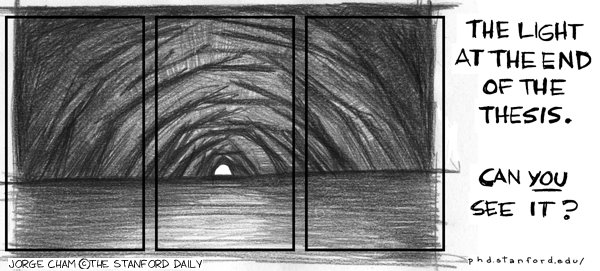
\includegraphics[width=.8\textwidth]{./gfx/Chapter07/phd051700s.jpg}
\caption{A descriptive comic strip by Jorge Chan from his series ``Piled Higher and Deeper'' \cite{ChamPhD}}
\end{figure}

The main goal of this thesis was to explore appearance-based methods in the novel contexts of wearable and hand-held object recognition and visual localization. As means to achieve this objective we collected two large datasets; provided a thorough evaluation of baseline and custom-created image description methods; developed a biologically inspired model of place cells for visual localization and produced a prototype system for assistive localization using wearable/hand-held visual input and tactile feedback.

In this final section we will briefly summarize each of these contributions and address some future perspectives.
\section{Summary of contributions}

\begin{enumerate}
\item \textbf{Proposal of a new approach} First, we have analysed the impact of computer vision in mobile and wearable technologies in an assistive context, providing complete studies of appearance-based methods for two key applications, hand-held object recognition of household products and indoor navigation.

\item \textbf{Artificial Place Cell Model} Second, we have provided a novel artificial place cell (APC) model for the biological counterparts found in the hippoccampus, and tested it under the same challenging conditions of indoor navigation by using a generalised regression neural network as a training mechanisms for learning a positional ground truth from a database.

\item \textbf{Prototype of an assistive application} Third, we took this previous findings to the next step and develop a prototype client-server Android application for assistive localization from wearable and hand-held devices using their visual input and a haptic feedback tablet to provide tactile cues to the location estimates.

\item \textbf{Two datasets} These contributions are accompanied by two important datasets, the SHORT dataset for hand-held object recognition and the RSM dataset of \emph{visual paths}.

\end{enumerate}

As we can see, from the computer vision application development pipeline devised in \ref{fig:cv_dev_pipeline} we have accomplished all the stages.

\section{Concluding remarks}

\section{Future work}

Finally, we will summarise here the future work for each line of work previously discussed briefly in each corresponding chapter.

\subsection{Datasets}

\subsubsection{SHORT dataset}

A large proportion of the time dedicated to the acquisition of SHORT was invested in prototypes of the acquisition set-up and trials for its testing. The intention was to have a flexible but at the same time reproducible set-up, as it can be shown in Fig. \ref{fig:acqsetup}. As the number of categories in the last version of SHORT, SHORT-100 was deemed appropriate in terms of generalisation under our testing conditions, we decided to stop its development there. However, the more categories we have in the training dataset the better for this type of benchmarks (controlled training set \textit{vs.} natural or \textit{wild} test set) to be adopted.

Regarding the test set, a natural expansion would consist of the setup of a web repository and the development of a retrieval mobile app so images of new grocery products could be contributed to the platform.

In this respect, there are open-source alternatives such as \cite{apple} and \cite{google} that would facilitate this task as instead of developing a dedicated app, the SHORT test set acquisition can be a project within these initiatives and attract altruist contributors that might have an interest on this sort of projects.

\subsubsection{RSM dataset}

The RSM dataset more corridors, different devices, and 2D ground truth.

\subsection{Appearance-based methods for visual localization}

\subsection{Biologically inspired localization methods based on place cell models}
Fisher Vector as method (GMM more biologically plausible?).
\subsection{Assitive localization apps with visual input and haptic feedback}


